\chapter{Hyperkinetic movement disorder analysis}
\label{ch:nemo}

\textit{
In this chapter, we present a real-world application for the dynamic projection methods introduced in \cref{ch:proj-eval,ch:proj-algo} in the context of hyperkinetic movement disorder analysis. These disorders manifest as abnormal involuntary movements that highly affect the quality of life of the people who suffer from them. These involuntary movements may present a wide range of tendencies: they may be regular and rhythmic, as in tremors; swift ``lightning-like'' jerks or twitches, as in myoclonus; sustained and repetitive movements resulting in abnormal postures, as seen in dystonia; they may present a random, brief, and non-rhythmic character, as in chorea; or can be temporarily suppressible jerks, as in tics.
The diagnosis of these disorders is carried out via careful professional observation. It can be extra challenging due to the circumstantial emergence of certain behaviors (trigged by specific postures or tasks) and their manifestation via compound movements, including a combination of the various hyperkinesias. All these factors lead to professionals often disagreeing with diagnosis. 
This chapter describes how we transform the data collected during clinical experiments, present our visual analytics tool, and show an example of data exploration that leads to valuable clinical insights using spectral analysis and temporal dimensionality reduction.
}

\vspace{5mm} %5mm vertical space


\eduardo{This in an initial report, not necessarily what the chapter/paper will look like. It is supposed to help me think about how to write about this project and guide me through preliminary patient data analysis.
\\
In the introduction and initial sections we will need to: \\
1 - introduce hyperkinectic movement disorders \\ 
2 - talk about how their manifestation in different people can differ wildly and how that makes them challenging to classify/diagnose even for medical specialists. \\
3 - talk about our goals creating this visual exploration tool and how this differs from a more traditional supervised learning approach. \\
\\
\\
After that we'll probably need a section introducing the different disorders and possibly explaining how they manifest in some of the tasks for illustration. \\
One thing that I'm not sure about is how familiar we expect the reader to be about these disorders.
\\
Then I think we should start to describe our contribution. And I would start by (1) describing the data itself and all the choices/transformations we make along the way until we get to the dynamic projection. 
\\
This includes: \\
\\
1 - Showing what the RAW data looks like \\
1.1 - General description of the experiment, including the tasks, sensor types, and possibly the different disorders (which must be introduced in a previous section). \\
1.2 - Show 3 axis accelerometer plot for 3 patients (e.g. healthy vs tremor vs chorea) \\
1.3 - Show spectrogram, interpret it, and talk about synchosqueezing \\ 
1.4 - Show how we get that spectrogram into a 'projectable' format: binning of the freqs + sliding window (width, stride) \\
1.5 - Show initial projections --  not sure what data to use here, maybe the 3 patients from before? Probably a more meaningful subset of the data would be better. Right now we have G-PCA, G-tSNE, and PCD-tSNE implemented. Explain dynamic projections and why they are useful and suitable for this application. Maybe do a trail vs single point comparison.
\\
\\
Next we need to move into data exploration, where we want to find examples of when dynamic projections can bring us insights into the data dynamics and the high dimensional space. Here we will be interested in looking for clusters, outliers, erratic/regular behaviour, failures in the data collection, etc.
\\ 
}

\eduardo{CODE: Check code to make sure I can switch sensors (DONE) and that I can 'stack' more than one sensor (NOT DONE))}

\noindent \textbf{Abstract:}

\section{Introduction}

\section{Related work}

\section{Hyperkinectic movement disorders and experiment design}

\section{Our approach}

Our goal was to design a visual analytics tool that supports exploring the motion data generated in the NEMO project. This is important given that the data is vast and has many axes that can be explored: there are over 100 patients, over 30 tasks, and 16 motion units which record accelerometer (3 axes), gyroscope (3 axes), and EMG (1 dimension) at up to 4370 samples per second, plus 3D video, and, for some experiments, page scans. 

Exploring this myriad of data is challenging. Thus, we aim to provide medical professionals with a tool to navigate and generate valuable insights from patient motion patterns effectively. For example, our tool must support a wide range of capabilities, such as identifying clusters, outliers, erratic observations, or failures in the data collection. It also must support medical analysis tasks, such as comparing various hyperkinesias to healthy behavior or identifying under which circumstances certain abnormal tendencies become incident. In both cases, we must be able to compare the severity and variability of their manifestation.

Another essential aspect is meta-analysis, where we want to know which combinations of sensors, tasks, patient groups, and preprocessing transformations generate representative data that may be useful in further investigation steps. Such meta-analysis is helpful if we want to build a classifier and keep only ``good data'' or if we want to understand the minimal resources (sensors and tasks) needed when performing data collection in a third-party clinic.

We envisioned a design that supports Shneiderman's mantra: overview first, zoom and filter, then details-on-demand. Nevertheless, to generate visualizations and interactions that implement these, we need to perform a series of transformations on the raw data, which are explained in detail next (\cref{fig:nemo-pipe}). 

\begin{figure*}[ht]
\centering
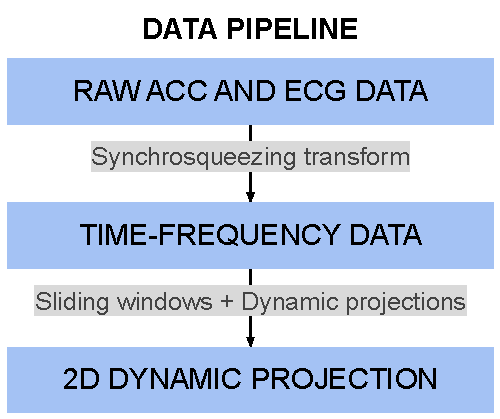
\includegraphics[width=.5\linewidth]{figures/nemo/simple-pipeline.pdf}
\caption{Data transformation pipeline.}
\label{fig:nemo-pipe}
\end{figure*}

To illustrate all the transformations, we begin by inspecting the raw data given by an accelerometer sensor placed on the subject's right hand. The task we will investigate is described as ``Arms stretched forward, wrists straight, palms down, and suppress involuntary movements'' (\cref{fig:hands}).

\begin{figure*}[ht]
\centering
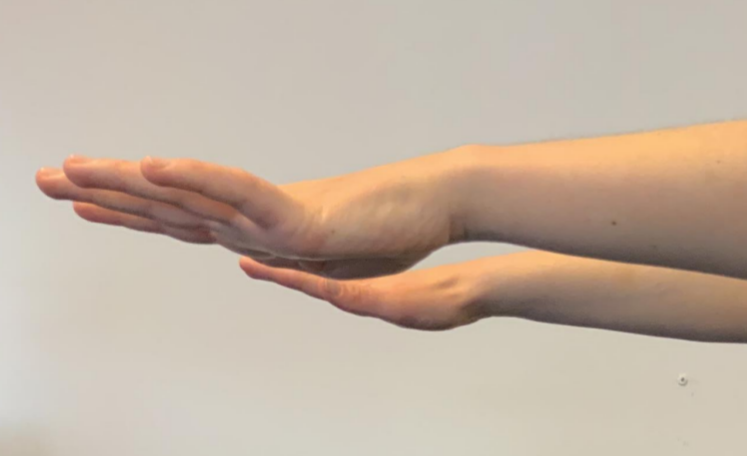
\includegraphics[width=.5\linewidth]{figures/nemo/hands.png}
\caption{Static position with arms and hands stretched out in front of body for 20-30 seconds. The subject tries to suppress any involuntary movements.}
\label{fig:hands}
\end{figure*}

\cref{fig:acc} shows the accelerometer data collected during the experiments for three subjects. For each subject, we see three colored lines corresponding to the X, Y, and Z axes measurements of a sensor placed on the right opisthenar (back of right the hand) recording at a rate of 148 samples per second. The lines are offset because the sensor reads the subject's movement acceleration and the Earth's gravity. An accelerometer at rest on the surface of the Earth will measure an upwards acceleration due to the gravity of $g \approx 9.81 m/s^2$. 

The same sensor unit also records gyroscopic and EMG data. We decided to ignore EMG data due to the additional complexity introduced in the non-standard preprocessing steps that (usually) involve noise rejection/filtering, whitening, gain scaling, demodulation, smoothing, and relinearization. For the next figures, we will only focus on accelerometer data.


On the three subplots of \cref{fig:acc} we see acceleration the data corresponding to three subjects: 
\begin{itemize}
  \item Patient \textit{a} is the healthy control: lines are not perfectly straight, indicating very low magnitude movement since it is impossible to hold this position perfectly still.
  \item Patient \textit{b}'s measurements show a very rhythmic and regular tremor of average magnitude for the disorder (\eduardo{can anyone check?}). This patient was diagnosed with essential tremor, the most common trembling disorder, often confused with Parkinson's disease.
  \item Patient \textit{c} was diagnosed with chorea and displayed high amplitude random non-rhythmic movements. \eduardo{Are we allowed to upload censored videos to a website?}
\end{itemize}
 

\begin{figure*}[ht]
\centering
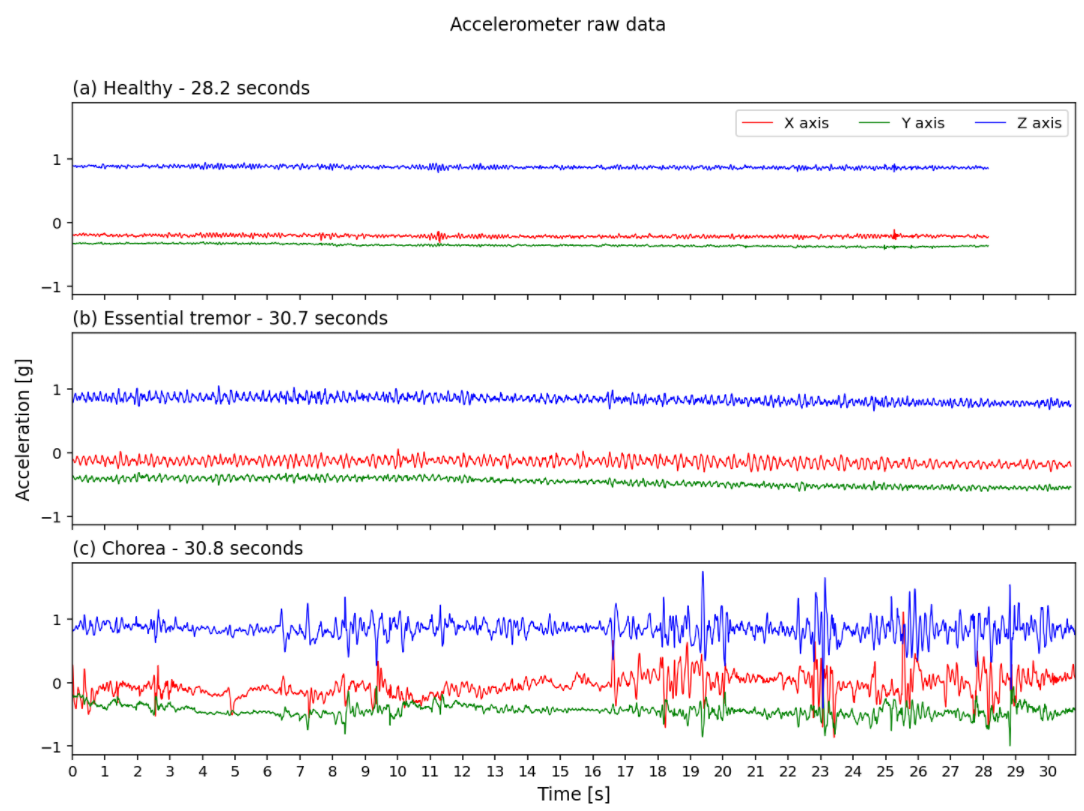
\includegraphics[width=\linewidth]{figures/nemo/acc2.png}
\caption{Accelerometer data for three subjects classified by experts as (a) healthy, (b) diagnosed with essential tremor, and (c) diagnosed with chorea. The data corresponds to a task where the subject must hold their hands as still as possible in the position suggested in Fig. \ref{fig:hands}.
Each subplot corresponds to the accelerometer data collected during the experiment and is broken down into three orthogonal components (X, Y, and Z-axis). \eduardo{Are we allowed to upload censored videos to a website?}}
\label{fig:acc}
\end{figure*}


These simple line graphs are handy for reasoning about the disorders and understanding their behavior over time. However, they do not tell the whole story. We can get a different perspective on the data that reveals relevant information hidden in the raw signal by decomposing it into the frequencies that form it. This can be done in two ways: with frequency-domain representation and time-frequency representation. The former assumes that the signal is stationary, which given the nature of our experiments, we know they are not, so we will not be using them. An example of a technique used in this case is the Fourier Transform. In contrast, time-frequency representation allows us to reason about how the frequency-domain (the spectrum) of a signal changes \textit{over time}.

The technique we use for time-frequency analysis is called Synchrosqueezing Wavelet Transform \eduardo{cite}. It is an improvement over the original Wavelet transform \eduardo{cite} which provides a sparser, sharper, noise-robust, and partly denoised representation of the time-frequency information. \eduardo{how deep do we want to go here?}

This time-frequency representation can be of great relevance for the diagnosis of motion disorders. For example, studies suggest that 95\% of essential tremor cases exhibited frequencies in the 5--8Hz range. If we examine \cref{fig:freq}(b), we can see that through the whole experiment, there is a defined presence of frequencies in this precise range, showing a common and insuppressible tendency to the involuntary movement. We don't see the same ``horizontal line'' in that frequency range for patients \textit{a} and \textit{c}. Patient \textit{a} can hold his/her hand in a much more stable position, which translates into a darker spectrogram (less energy). In contrast, patient \textit{c} performs high amplitude random non-rhythmic movements characteristic of chorea. The light colors in the spectrogram represent the high amplitude, and the ``random non-rhythmic'' aspect can be read as having no constant lines in the time-frequency representation, as seen on patient \textit{b}. Having both representations (\cref{fig:acc,fig:freq}) side-by-side helps us understand the phenomena as a whole. 
% https://www.ncbi.nlm.nih.gov/pmc/articles/PMC3475963/

For our purposes, the time-frequency representation is essential as it facilitates comparison between signals. Methods for computing similarity of signals in the time-domain (raw signals) exist (such as RMSE, cross-correlation, and Dynamic Time Warping \eduardo{cite all}). However, these can be significantly affected by the phase shift and minor differences in frequency. By making comparisons in the time-frequency domain, we get a better, more reliable representation that is better suited for the next steps of the pipeline.

%The sensor reads acceleration in three orthogonal axes (X, Y, Z). For the next figures, we will focus on the Z axis, which points up/down for the hands shown in \cref{fig:hands}.

\begin{figure*}[ht]
\centering
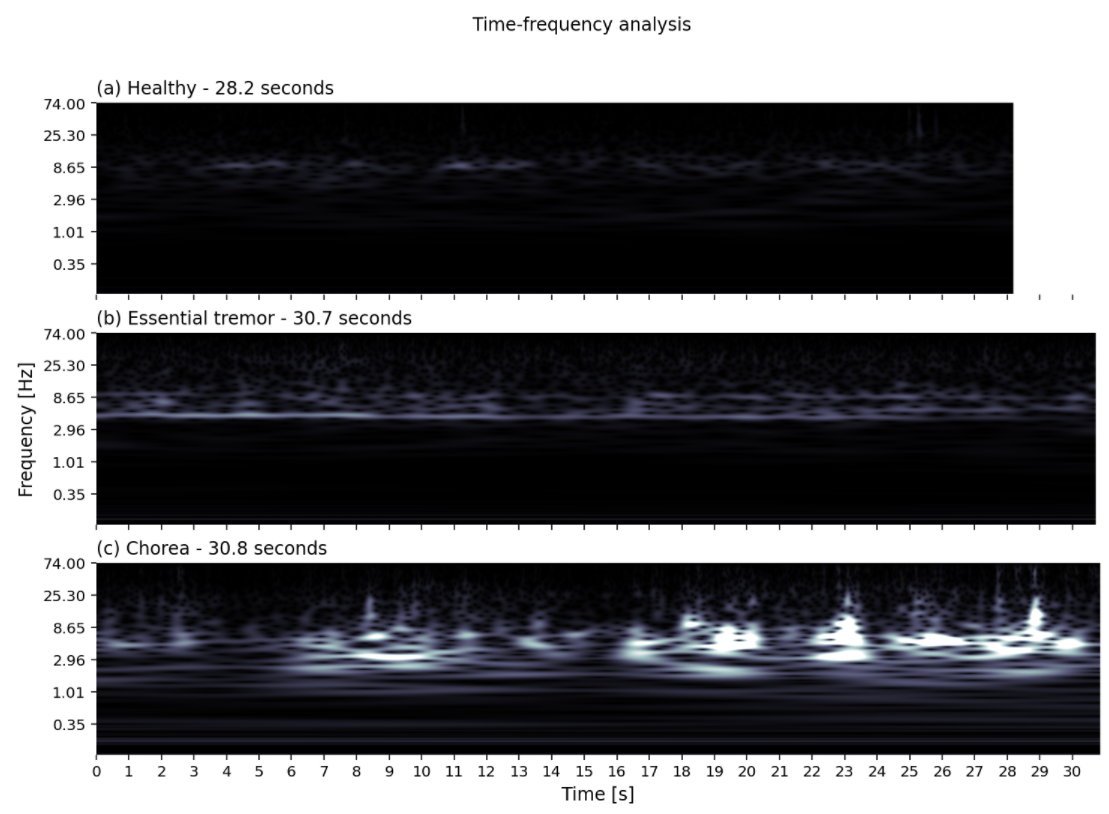
\includegraphics[width=\linewidth]{figures/nemo/freq2.png}
\caption{Time-frequency representation of the acceleration of the Z axis (blue) in Fig. \ref{fig:acc}. This is the vertical axis which points up/down for the hands shown in \cref{fig:hands}. Light colors represent high energy in the spectral distribution, i.e., there is a large amplitude component in the subject's movement associated to a particular frequency or frequency distribution. \eduardo{add colormap}}
\label{fig:freq}
\end{figure*}

Before we project our data, we need to get it in a uniform and easily comparable format. As seen in \cref{fig:freq}, time-frequency information can vary slightly from recording to recording: they have different lengths and different frequency precision. Both of these are due to the difference in experiment duration. Experiments that last more have longer spectrograms and higher frequency definition since we can detect more frequencies in the lower range. The sampling rate of the sensor sets the upper range of the frequency spectrum. The accelerometers we used can collect 148 readings per second, so the maximum frequency we can detect is 74 Hz. We also limit our frequency range to 100 logarithmic bins in the range of $0-74$ Hz. 

To get our data in this uniform and easily comparable format, we use the Sliding Window method as illustrated in \cref{fig:sliding}. In this example, we set a stride of 1 second and a window width of 5 seconds. One additional advantage of using this method is that we can change the parameters on the fly to generate projections of different ``resolutions'', as seen on \cref{fig:nemo1-projections}. What is meant by resolution is the number of points (which connected create a polyline) that represent a recording in the projection.


\begin{figure*}[ht]
\centering
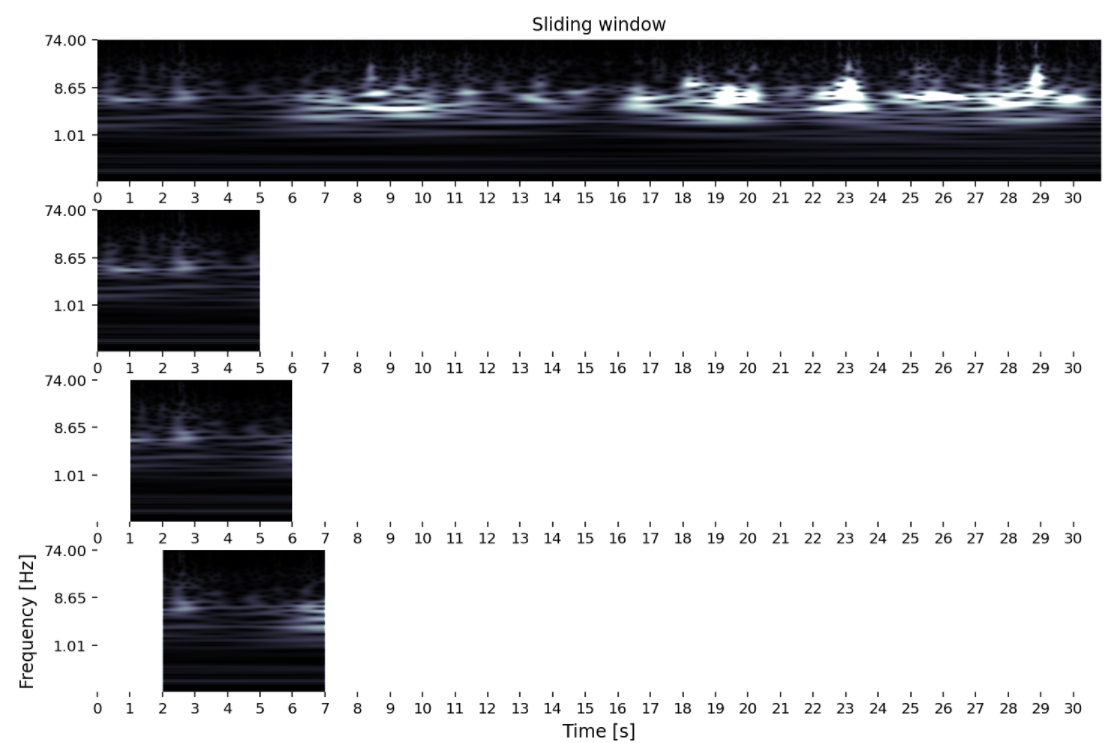
\includegraphics[width=\linewidth]{figures/nemo/sliding.png}
\caption{Before we project our data, we subdivide each spectrogram using the Sliding Window method. In this example, we use a window width of 5 seconds and a stride of 1 second to partition the data from Fig. \ref{fig:freq}c.}
\label{fig:sliding}
\end{figure*}

Since our data is multidimensional and temporal, we use dynamic projections to obtain further insights into our dataset.
For this prototype, we implemented three of the dynamic projection methods introduced in the previous two chapters. These are G-PCA, G-tSNE (\cref{ch:proj-eval}), and PCD-tSNE (\cref{ch:proj-algo}). 
G-PCA and PCD-tSNE are methods that balance visual quality and temporal stability, but they each have pros and cons. PCD-tSNE has better neighborhood and distance preservation than G-PCA and comparable stability. Its main drawback for this particular application is that a few parameters need to be adjusted, which adds an undesired level of uncertainty when interactively exploring the data. This same trait outside of an interactive setting can be advantageous, as it allows us to create projections that borrow characteristics from both PCA and tSNE-based methods, as previously discussed in \cref{sec:results}. % chapter 6
G-tSNE is a relatively unstable technique, as benchmarked in \cref{ch:proj-eval}. However, it still provides interesting (non-temporal) insights into the high-dimensional structure of the data.

\cref{fig:nemo1-projections} shows the data from patients \textit{a}, \textit{b}, and \textit{c} projected using the three methods. Because the spectral signatures of the different patients are different from each other, we see that the trails do not overlap. We also observe how PCD-tSNE creates a projection that borrows traits from both G-PCA and G-tSNE. The general position of all clusters and shape of the (c) trail resemble that of G-PCA, while the focus on intercluster neighborhood preservation for trails (a) and (b) (materialized as expanded clusters) are traits derived from the tSNE influence.

\begin{figure*}[ht]
\centering
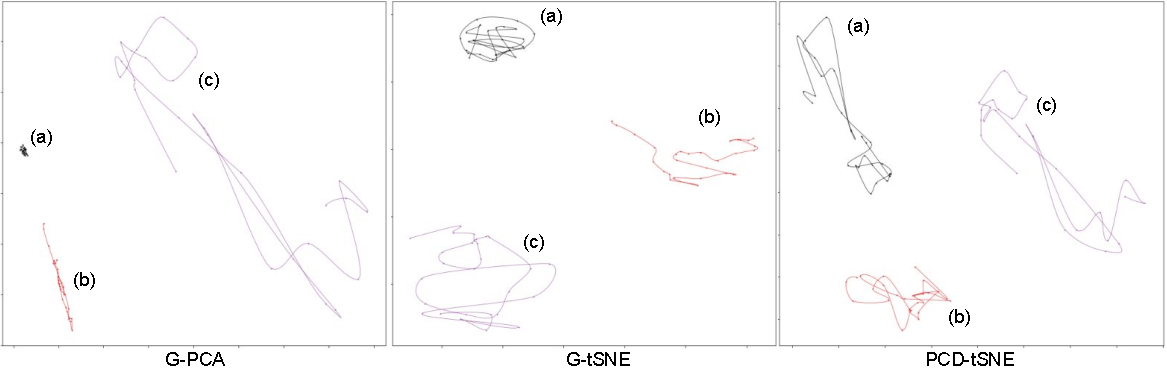
\includegraphics[width=\linewidth]{figures/nemo/nemo1-projections.pdf}
\caption{The last step of the pipeline is to project (using dynamic methods) the data that has been subdivided by the Sliding Window method. Our tool supports 3 dynamic projection methods: G-PCA, PCD-tSNE, and G-tSNE. We visualize the dynamic projections as trails, where we connect the consecutive spectrum ``windows'' via Akima spline \eduardo{cite}. The data corresponds to the patients presented in \cref{fig:acc,fig:freq}.}
\label{fig:nemo1-projections}
\end{figure*}

\section{Data exploration}

This section presents an example of the kind of data exploration that our tool supports. The NEMO project has over 100 participants diagnosed with six different disorders \eduardo{how many?}. Each participant performed over 30 tasks whiled being measured by tens of sensors.

There are many ways to conduct data exploration, depending on the goal of the analysis. Some relevant examples from a clinical standpoint are:
\begin{itemize}
  \item Understand the behavior of different patients or patient groups for a given task; 
  \item Given new patient measurements, find patients with similar movement characteristics to assist diagnosis;
  \item Explore the movements that led to a specific diagnosis;
  \item Study the erratic/circumstantial nature of the appearance of certain symptoms;
  \item Understand how different tasks induce different behaviors on specific patients or patient groups. 
\end{itemize}

In the following analysis, we will perform an example analysis that will focus on the first goal. We want to understand the behavior of essential tremor patients \textit{vs} healthy controls in the context of the task described as ``arms stretched forward, wrists straight, palms down, and suppress involuntary movements'' (\cref{fig:hands}). In total, we have 24 healthy subjects and 11 tremor patients.
For the next figures, we will use the reading from the Z-axis of the accelerometer sensor placed on the subject's right hand. Our tool supports interactive real-time change of all the filters set above.

Once we selected the data subset of interest, we need to choose how to project the data. \cref{fig:exp1-gpca} displays two G-PCA projections. The only difference is the size of the sliding window (\cref{fig:sliding}), which translates into the resolution and smoothness of the projection. The left projection has a sliding window size of 1 second and a stride of 1 second, meaning that there is no overlap between the consecutive windows, leading to more jagged trails. The right projection has a window size of 5 seconds instead, so consecutive windows share part of the same data, leading to a longer representation of temporal phenomena and smoother lines. Choice of windows size and stride also depends on the amount of data we are projecting, i.e., number of patients and length of experiments. We will use a window size of 5 seconds and a stride of 1 second for the following figures. 

\begin{figure}
\centering
\begin{minipage}{.5\textwidth}
  \centering
  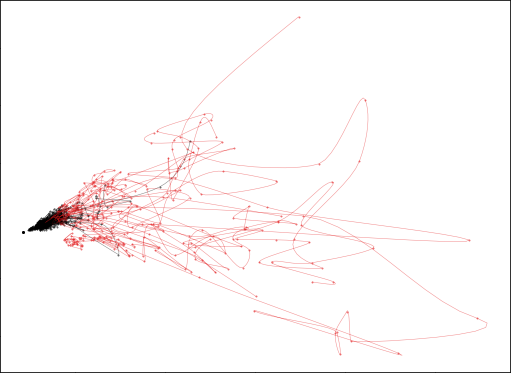
\includegraphics[width=\linewidth]{figures/nemo/exp1.png}
  % \captionof{figure}{A figure}
  % \label{fig:exp1-gpca-1s-1s}
\end{minipage}%
\begin{minipage}{.5\textwidth}
  \centering
  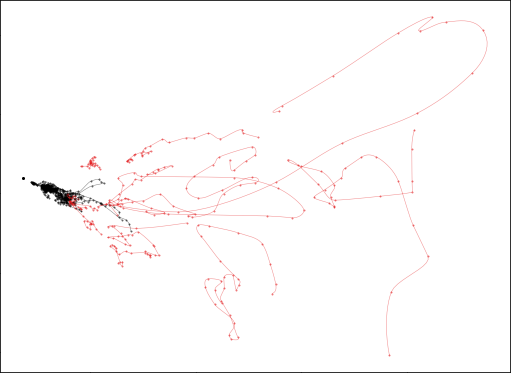
\includegraphics[width=\linewidth]{figures/nemo/exp1-5s-window.png}
  % \captionof{figure}{Another figure}
  % \label{fig:exp1-gpca-5s-1s}
\end{minipage}
\caption{G-PCA projection of 24 healthy (black) and 11 tremor (red) patients with window width and stride of [1s, 1s] on the left and [5s, 1s] on the right.}
\label{fig:exp1-gpca}
\end{figure}


With the projected data in front of us, we can start making some assumptions. For example, we see that most healthy patients (black trails) cluster together in a tight formation in the ``center'' of the projection, while the tremor patients' trails tend to be located to the right of this cluster and with a broader spread. The angle and distance from the central cluster must portray some traits in the data, but we cannot confirm anything just yet.   

To better understand the overall structure of the projection, we can start by looking at a couple of trails drawn in its periphery. We start selecting patient 91 (\cref{fig:exp1-9196}-left). Our tool also displays the video recording of the experiment, but we do not show it due to privacy concerns. 

Patient 91 presents a unique behavior. Looking at the raw signal and spectrogram, we can tell that in the initial 2-3 seconds, there is a presence of medium amplitude tremors, followed by high amplitude tremors until 13s, and then a significant reduction in the intensity until the end of the experiment. We also see that the movement is decomposed into a ``sharp'' spectrum, mainly focused on around 5 Hz. Without talking to the patient, we can only speculate. However, one hypothesis is that the patient can suppress involuntary movements after considerable effort, which is only possible after a few seconds into the experiment. This dynamic translates in a particular projection trail (top-left): it starts a certain distance away from the center of the projection, characteristic of ``unhealthy'' behavior, and then ``shoots'' away to the top left as tremor intensity increases, only to finally move closer to the center of the projection, close to the healthy cluster as the amplitude is reduced. This hints that the distance from the ``center'' of the projection is related to the energy in the signal, that is, how large the movements are. 

The three plots on the right portray the data collected from patient 96 (\cref{fig:exp1-9196}-right). This patient was also diagnosed with important tremors, but its manifestation shows essential differences compared to patient 91's. Patient 96 shows a more constant tremor. Its amplitude is constantly high, showing that the patient cannot suppress the movement. Another dissimilarity comes in the signature of the tremor: Patient 91 has a ``sharp'' histogram, meaning that his tremor has very sinusoidal tendencies, while the same is not valid for patient 96, given the presence of high energy high frequencies on the spectrum. Upon detailed inspection of the video recording, this can be related to the fact that patient 96's tremor has a more lateral tendency (side-to-side instead of up-and-down). \eduardo{check} We also notice extra movement at the beginning of the recording as the patient gets into position, which can be identified in the projection as abnormal movements that make the trails start at the right-bottom at a considerable distance from where the rest of the trail is located.  

\begin{figure*}[ht]
\centering
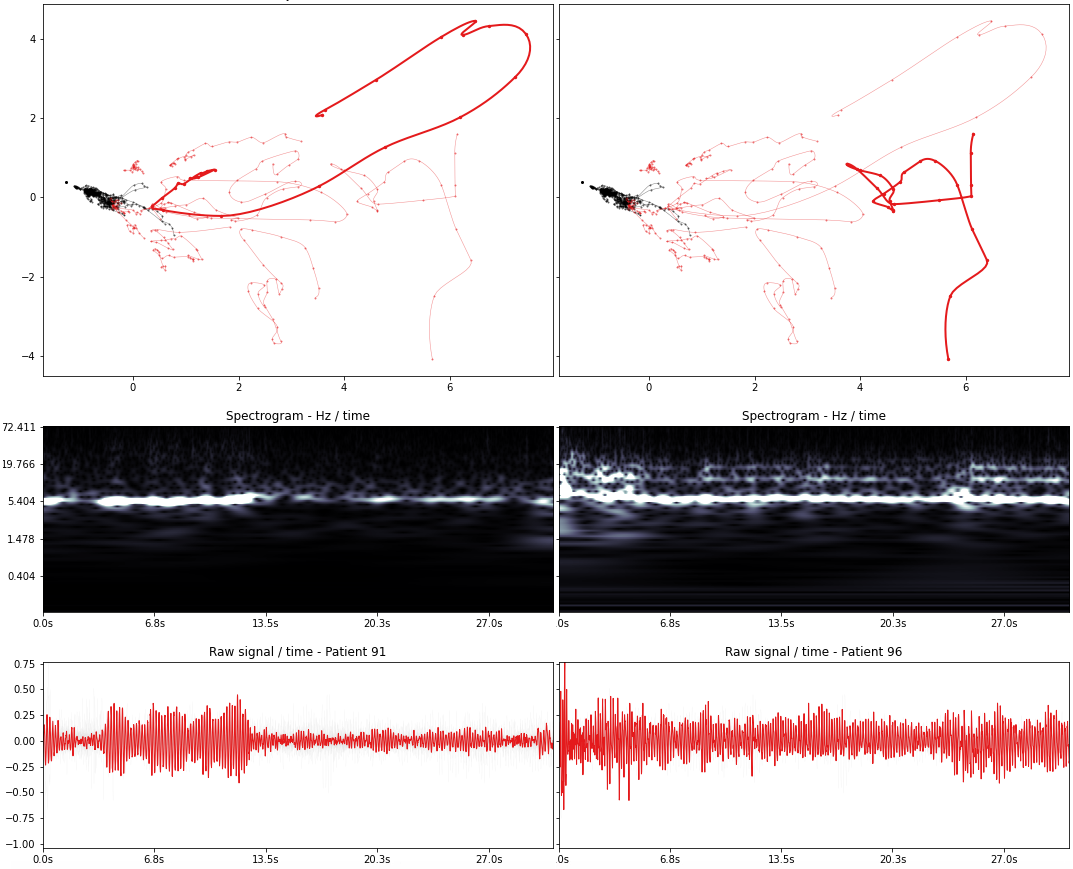
\includegraphics[width=\linewidth]{figures/nemo/exp1-9196.png}
\caption{Our tool allows selection and inspection of patients. Other than the plots shown in the figure, the tool also displays a video recording of the experiment. \eduardo{do we have to hide the patient ids (91 and 96)? }}
\label{fig:exp1-9196}
\end{figure*}

The projection also allows us to investigate the border between the two classes, potentially revealing subjects of interest with complex diagnoses.
\cref{fig:exp1-3942} shows two subjects whose trails are in the border and overlap each other. However, patient 39 (left) is classified as healthy, while patient 42 (right) was diagnosed with essential tremor. Comparing their signals, we see that subject 39's signal has a larger amplitude and a sharper spectrum, which to the untrained eye, it could mean that he/she suffers from tremors. However, the subject's tremors have a very high-frequency main component (over 10 Hz), which puts him/her outside the normal range for essential tremors (5--8 Hz) -- maybe the subject just drank too much coffee in the morning. His/her tremor also does not seem to be a very significant impact on other tasks. Patient 42, however, does not display obvious tremor symptoms in this particular static task, but given its classification, we must explore the reasons for the diagnosis.
Further exploration tells us that this particular patient has one side of the body more affected than the other. The condition appears to be more noticeable when performing active tasks (instead of holding static positions), as witnessed by the Archimedes Spiral tests (\cref{fig:spirals}). Patient 42 shows tremor signals for both hands, but the tremor is much more apparent on the left.

\begin{figure*}[ht]
\centering
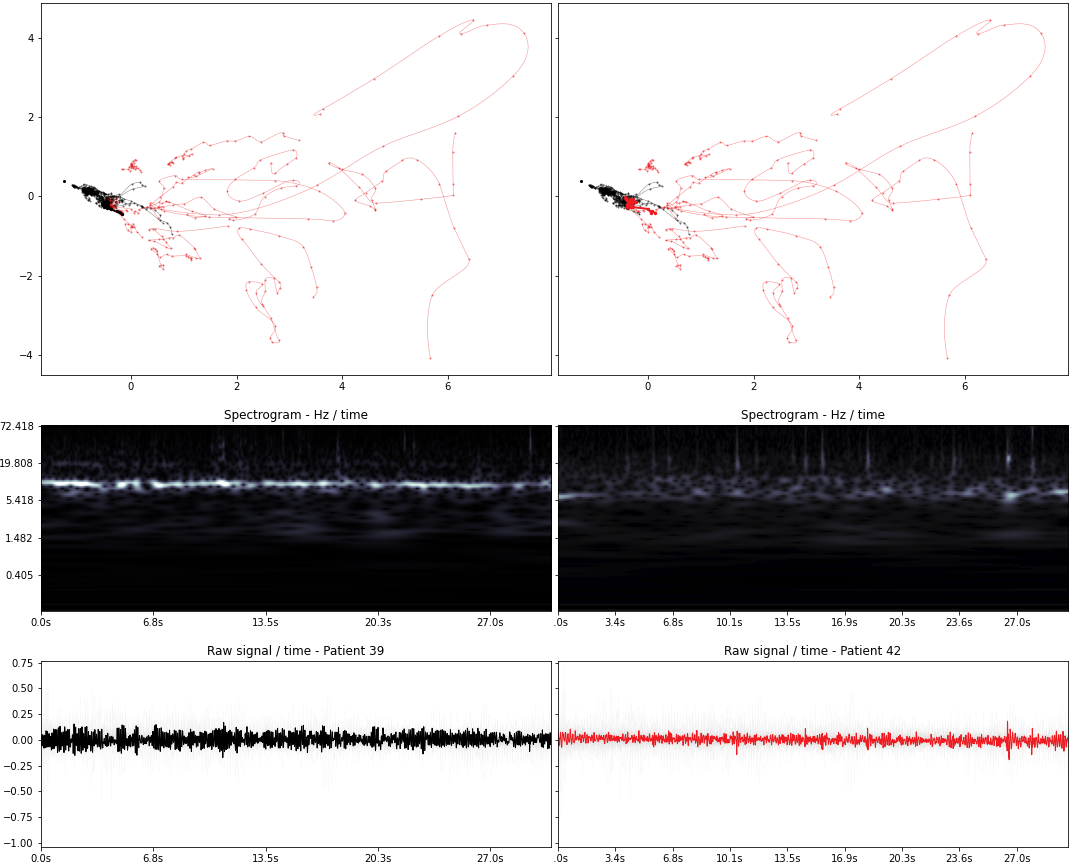
\includegraphics[width=\linewidth]{figures/nemo/exp1-3942.png}
\caption{The trail representing the patient on the right is very close to the healthy group. If we look at only his right hand during the recording of this specific task, it is hard to tell that he/she suffers from tremors, and it raises the question as to why was he/she diagnosed with tremors. Does it have a postural/unilateral aspect that is not captured in this task? \eduardo{hard to see, not sure how I can make it better.}}
\label{fig:exp1-3942}
\end{figure*}

\begin{figure*}[ht]
\centering
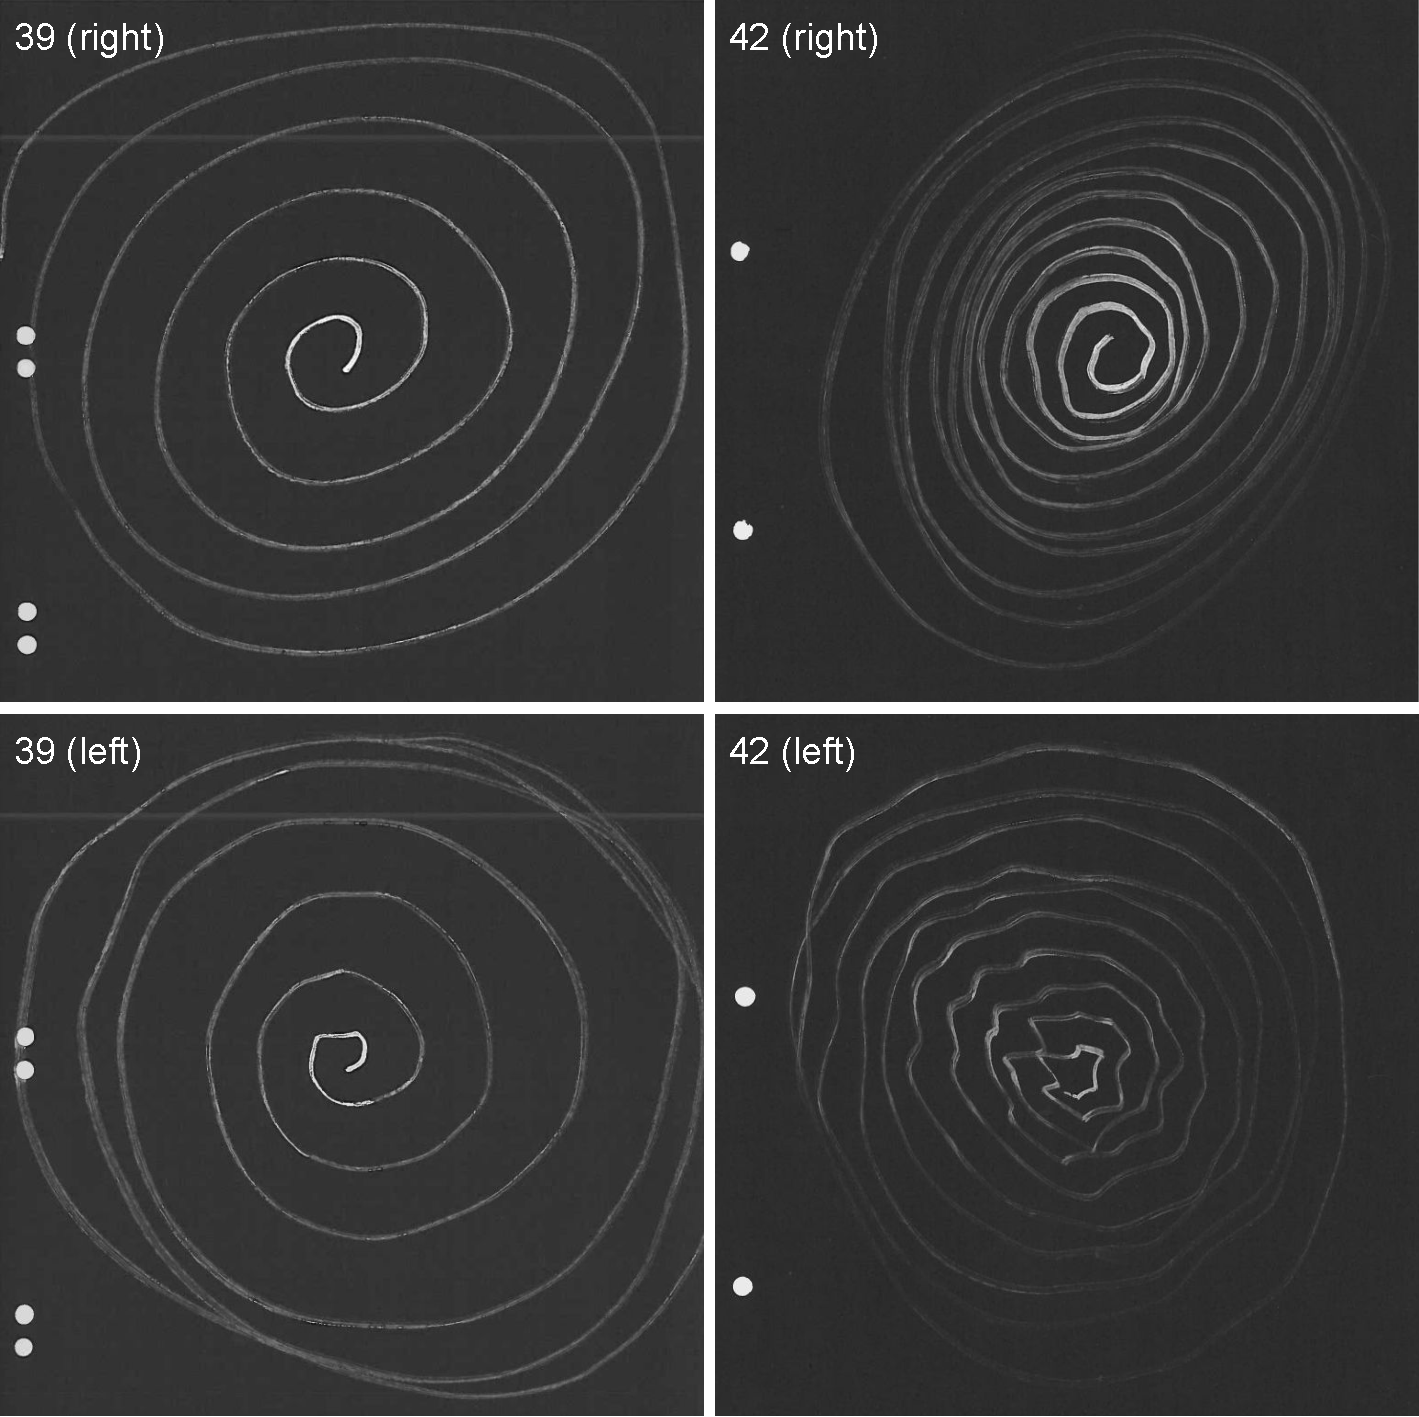
\includegraphics[width=.7\linewidth]{figures/nemo/4-spirals.pdf}
\caption{Archimedes spirals for both hands of patients 39 and 42.}
\label{fig:spirals}
\end{figure*}
    
Lastly, we can notice some healthy trails reaching out into ``tremor territory'', revealing interesting subjects for investigation. One trail that attracts attention in the projection is the one of patient 3 (\cref{fig:exp1-337}-left). While most of the trail is located near other healthy patients, a part of the trail extends to the right. Looking at the spectrogram and raw signal, we can see that the patient trembles for a short period. However, the video shows that this happens as the patient talks to the researchers and slightly moves its legs, which does not indicate an incorrect diagnosis.
Such a trail could also mean that a true essential tremor patient lost control of the suppression of the involuntary movement. The moment this happens is clearly pointed out in the projection and could have been easily not noticed in a clinical setting. We see a similar trend for patient 37 (\cref{fig:exp1-337}-right), but in this case, the movement is due to a late stop of the recording -- the sensors and camera keep going as the subject is told to return to a rest position. These recordings also help us confirm an earlier suspicion about the meaning of the northeast and southeast portions of the projection space. These are related to the ``sharpness'' of the spectrum: signals where the frequency band of 5--8 Hz tends to form the majority of the spectrum energy tend to go north-east, these ``well-behaved/well-defined'' tremors. At the same time, the direction towards the southeast of the projection is representative of more uniform spectral distributions, related to more chaotic movements.

\begin{figure*}[ht]
\centering
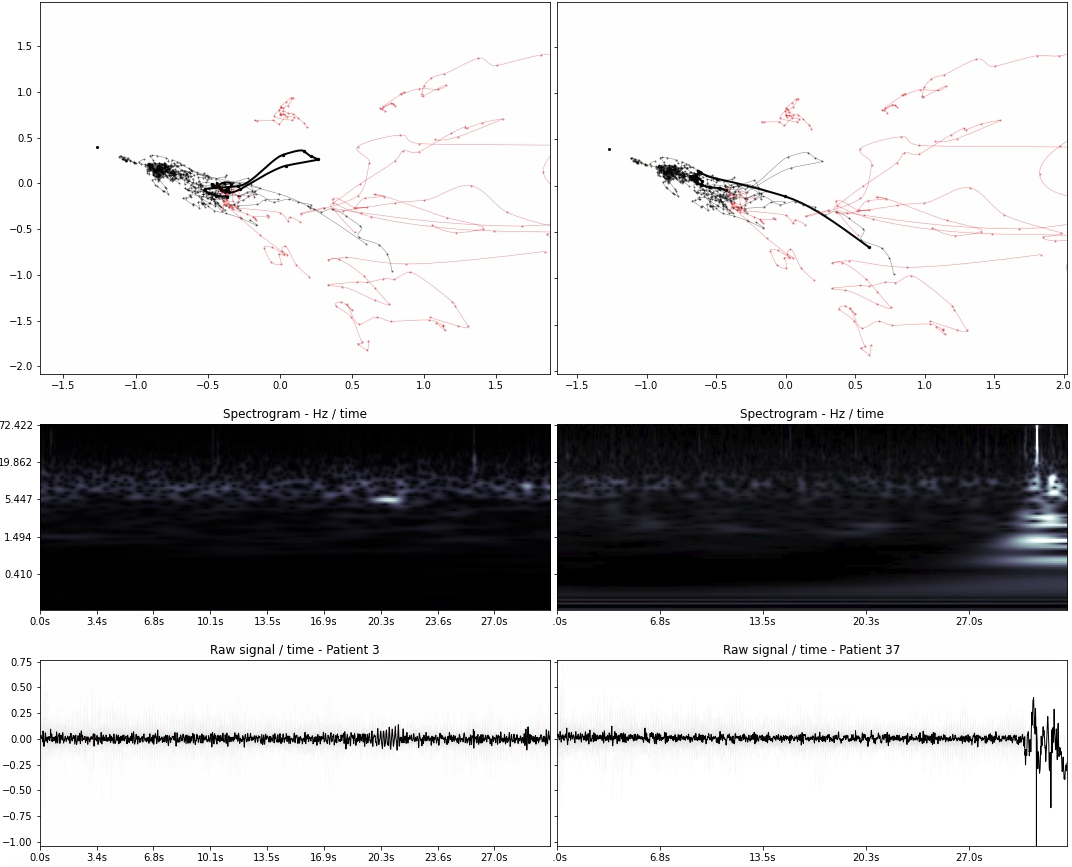
\includegraphics[width=\linewidth]{figures/nemo/exp1-337.png}
\caption{Temporary tremors on the left, and premature end of experiment on the right.}
\label{fig:exp1-337}
\end{figure*}

All the previous analysis was done atop of a single G-PCA projection. However, the other methods implemented into the tool might offer different perspectives on the data, which could be useful in other tasks. \cref{fig:diff-projs} shows 6 projections of the same data. These projections show a  PCD-tSNE characteristic previously discussed (\cref{sec:lambda}), in which it proves itself capable of evoking traits from PCA (focus on distance preservation) and tSNE (focus on neighborhood preservation) based on the setting of the $\lambda$ parameter.

\begin{figure}
\begin{tabular}{cc}
\subfloat[G-PCA]{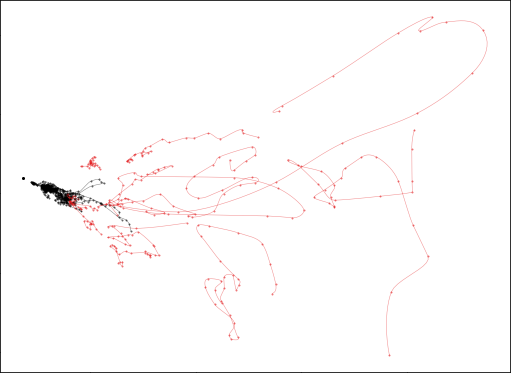
\includegraphics[width=.5\linewidth]{figures/nemo/exp1-5s-window.png}} &
\subfloat[PCD-tSNE $\lambda=.1$]{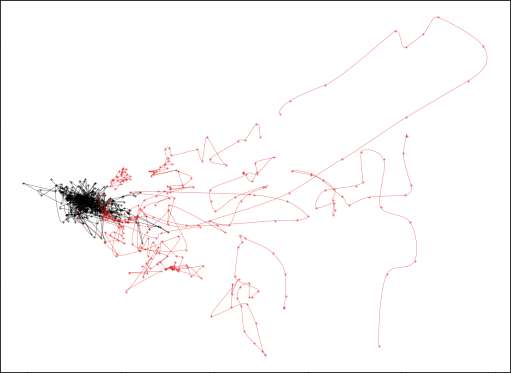
\includegraphics[width=.5\linewidth]{figures/nemo/exp1-pcd0,1.png}} \\
\subfloat[PCD-tSNE $\lambda=.001$]{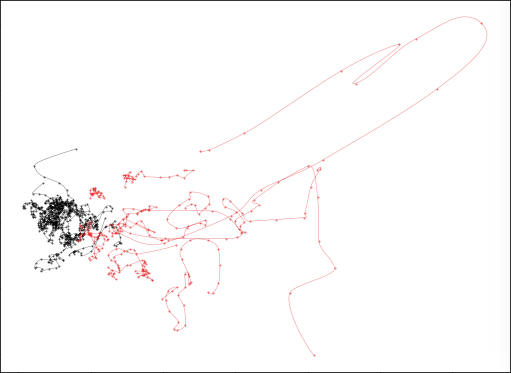
\includegraphics[width=.5\linewidth]{figures/nemo/exp1-pcd0,001.png}} &
\subfloat[PCD-tSNE $\lambda=.0001$]{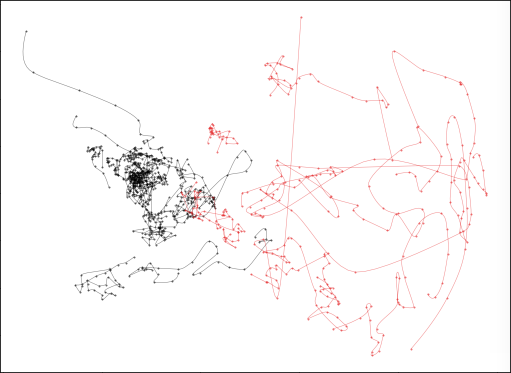
\includegraphics[width=.5\linewidth]{figures/nemo/exp1-pcd0,0001.png}}\\
\subfloat[PCD-tSNE $\lambda=.000001$]{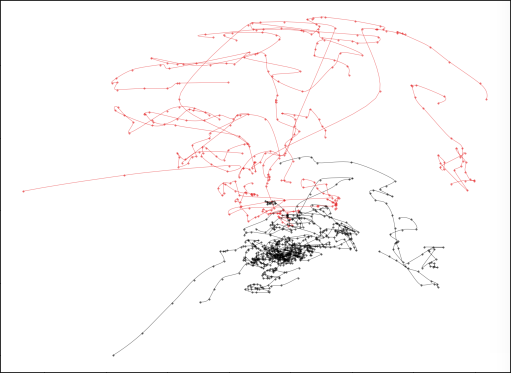
\includegraphics[width=.5\linewidth]{figures/nemo/exp1-pcd0,000001.png}} &
\subfloat[G-tSNE]{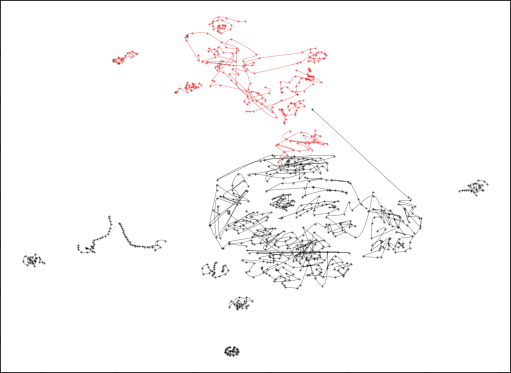
\includegraphics[width=.5\linewidth]{figures/nemo/exp1-gtsne.png}}
\end{tabular}
\caption{Different projection of the same data showing how PCD-tSNE is able to create a hybrid focus on distance preservation or neighborhood preservation depending on the $\lambda$ parameter setting.}
\label{fig:diff-projs}
\end{figure}


\section{Discussion}

% right now we are only doing task-wise analysis, maybe we want to change the focus to the analysis of a given patient given what we know is normal and abnormal behaviour.

\section{Conclusions}


    
